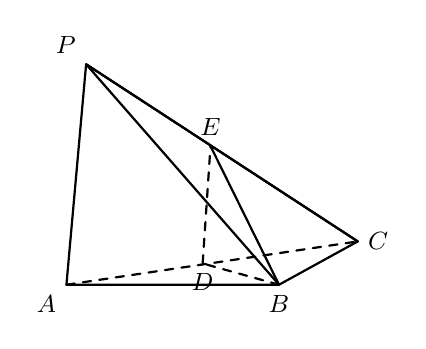
\begin{tikzpicture}[thick,line cap=round,line join=round,
  every node/.style={font=\small}]
  \coordinate (P) at (0,2.8);
  \coordinate (A) at (-.25,0);
  \coordinate (B) at (2.45,0);
  \coordinate (C) at (3.45,.55);
  \coordinate (D) at (1.48,.27);
  \coordinate (E) at (1.58,1.76);
  \draw (P)--(A)--(B)--(C)--(P)--(B);
  \draw (P)--(C);
  \draw[dashed] (A)--(C);
  \draw (B)--(E);
  \draw[dashed] (D)--(E) (B)--(D);
  \node[above left] at (P) {$P$};
  \node[below left] at (A) {$A$};
  \node[below] at (B) {$B$};
  \node[right] at (C) {$C$};
  \node[below] at (D) {$D$};
  \node[above] at (E) {$E$};
\end{tikzpicture}
